%
\section{Software specification}
\label{sec:sw-specs}
Next, the \gls{sw} responsible for system operation is specified for all
subsystems --- \texttt{\gls{mdo-rc}}, \texttt{\gls{mdo-rs}}, and
\texttt{mdo-l}.
All these subsystems are event-driven (asynchronous), and they can be more easily
specified using state-machine diagrams, previously illustrated in the
\emph{analysis phase} (Section~\ref{sec:softw-arch}). Also in the \emph{analysis
phase}, the use case diagrams helped to identify the main features required for
the system and the respective sequence diagrams helped to clarify the
intervening objects and the interaction among them.

In this section, the analysis phase information is used to derive the static
architecture of the system --- classes diagram --- and to specify algorithms for
its implementation through flowcharts, keeping in mind that the several
subsystems operate multiple tasks concurrently, thus requiring the tasks'
specification and its priorities. The data frame formats are specified for
communication between the different modules. The \acrfull{erd} are depicted to
design the required databases and the \gls{ui} mock-ups are recalled. The test
cases for each subsystem are listed, defining its operation and the expected
result. The \gls{cots} \gls{sw} and the third-party libraries are identified
and a mapping between class topics and the foreseeable implementation is
presented for clarification. Finally, the \gls{sw} tools are listed.

\subsection{Software architecture}
\label{sec:softw-arch-1}
The system's \gls{sw} architecture was devised using \emph{\gls{uml} component
  diagrams} for \texttt{Remote Client} (Fig.~\ref{fig:component-diag-rc}), \texttt{Remote Server} (Fig.~\ref{fig:component-diag-rs}), and
\texttt{Local System} (Fig.~\ref{fig:component-diag-local}). Each component
diagram illustrates all \gls{sw} components for the system in analysis and the
interaction between them, and its
interfaces with external subsystems.

\subsubsection{Remote client}
\label{sec:remote-client-arch}
The \texttt{Remote Client} \gls{sw} architecture is comprised of the following
artifacts:
\begin{itemize}
\item
  \emph{\texttt{User Interface} package}: contains the \texttt{\gls{ui}} and \texttt{\gls{ui} Engine}
\item
  \emph{\texttt{Comm Manager} package}: 
\item
  \emph{\texttt{DB Manager} package}:
\item 
  \emph{\texttt{Remote Controller} package}:
\item
  \emph{\texttt{RC Rx Parser} component}:
\item
  \emph{\texttt{\gls{tcp-ip} Tx} socket}:
\item 
  \emph{\texttt{\gls{tcp-ip} Rx} socket}:  
\end{itemize}

\begin{figure}[htb!]
\centering
    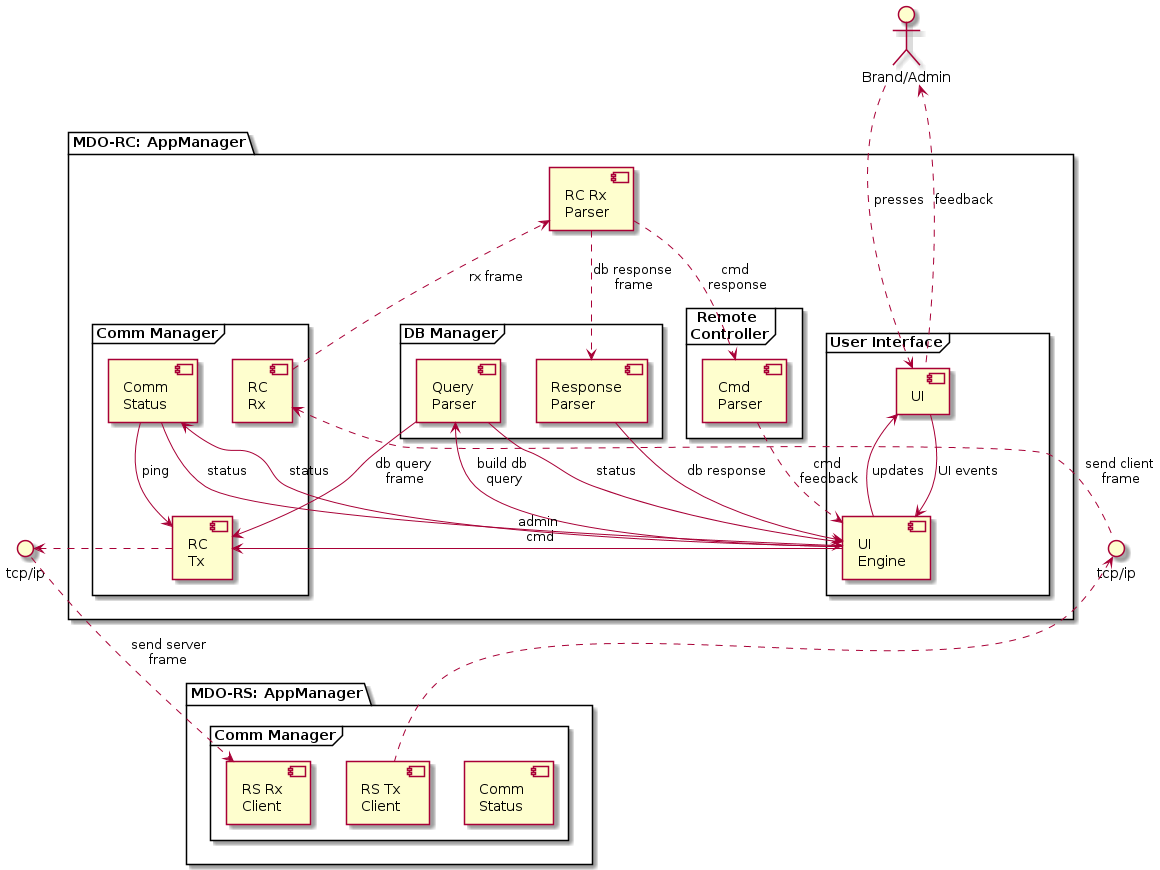
\includegraphics[width=0.9\columnwidth]{./img/component-diag-rc.png}
  \caption{\gls{sw} architecture: component diagram --- \texttt{Remote Client}}%
\label{fig:component-diag-rc}
\end{figure}

\subsubsection{Remote server}
\label{sec:remote-server-arch}


\begin{figure}[htb!]
\centering
    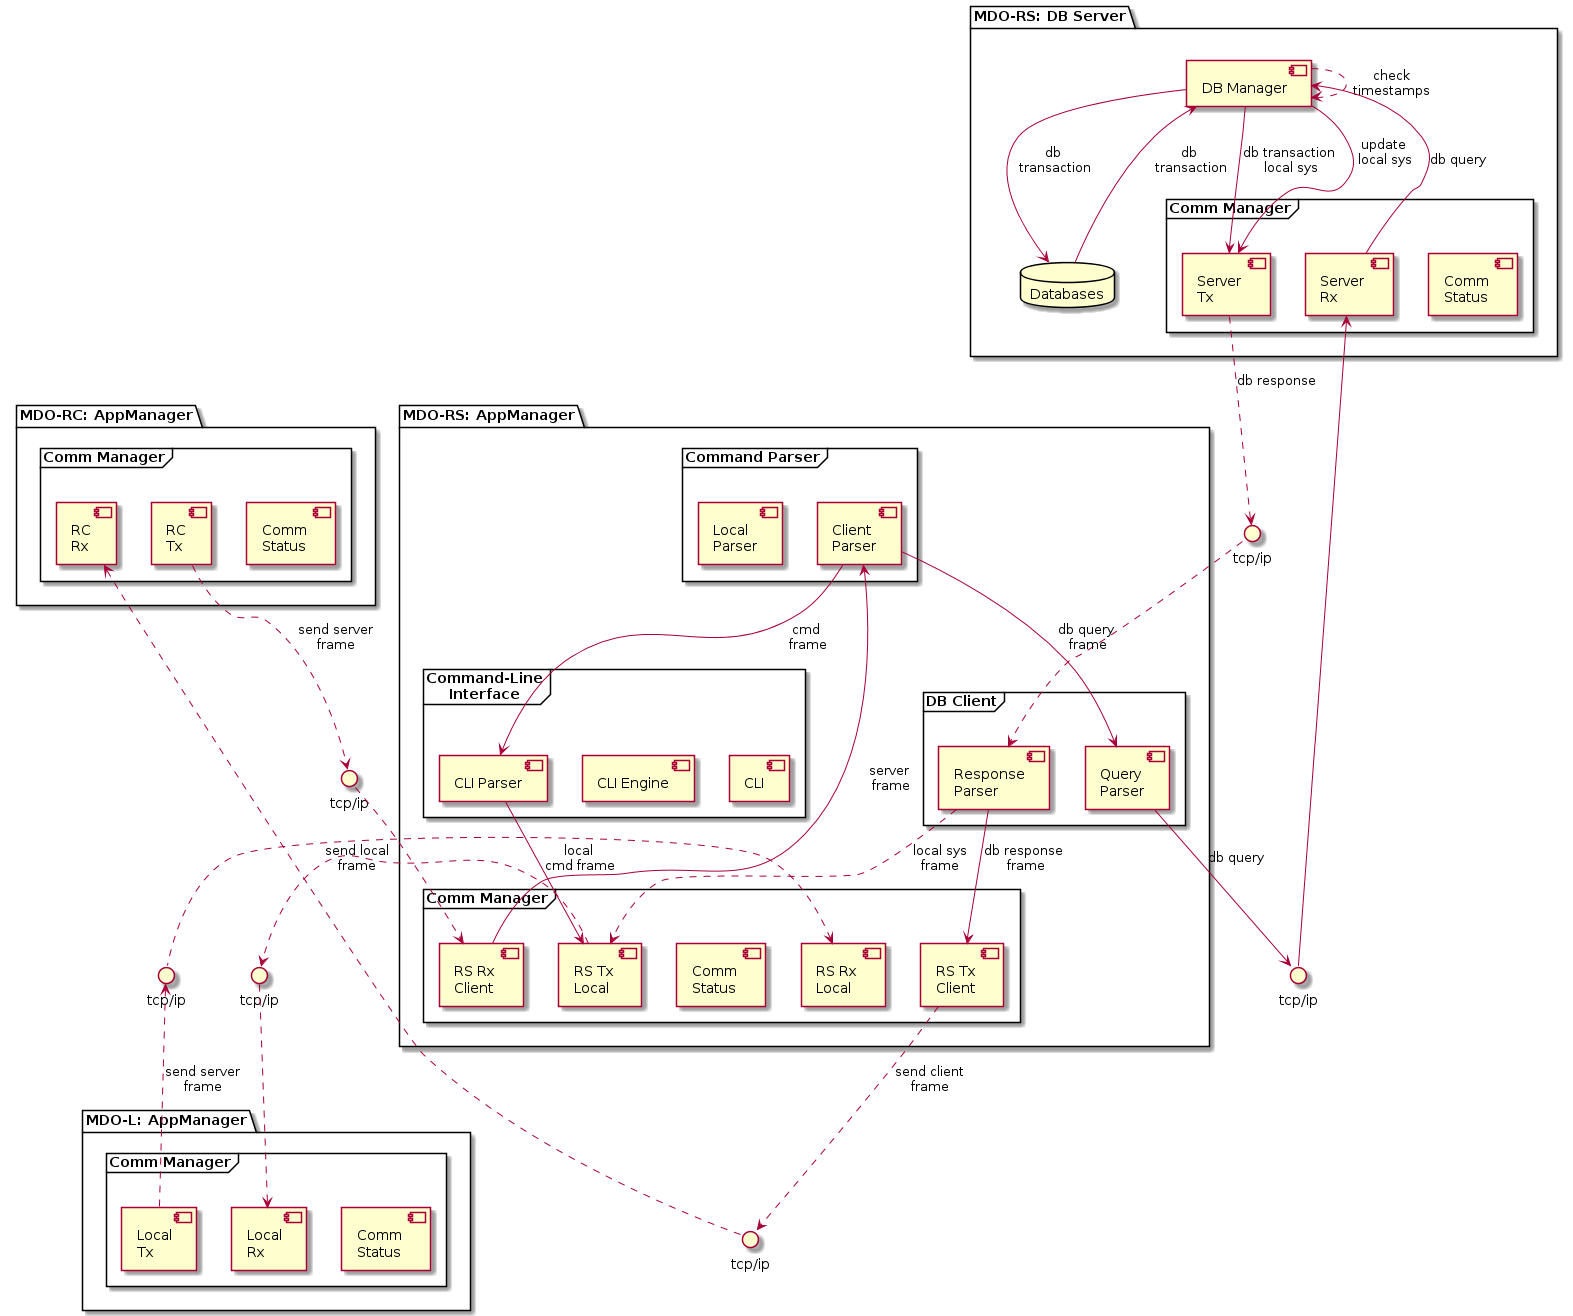
\includegraphics[width=0.9\columnwidth]{./img/component-diag-rs.png}
  \caption{\gls{sw} architecture: component diagram --- \texttt{Remote Server}}%
\label{fig:component-diag-rs}
\end{figure}

\subsubsection{Local system}
\label{sec:local-system-arch}

\begin{figure}[htb!]
\centering
    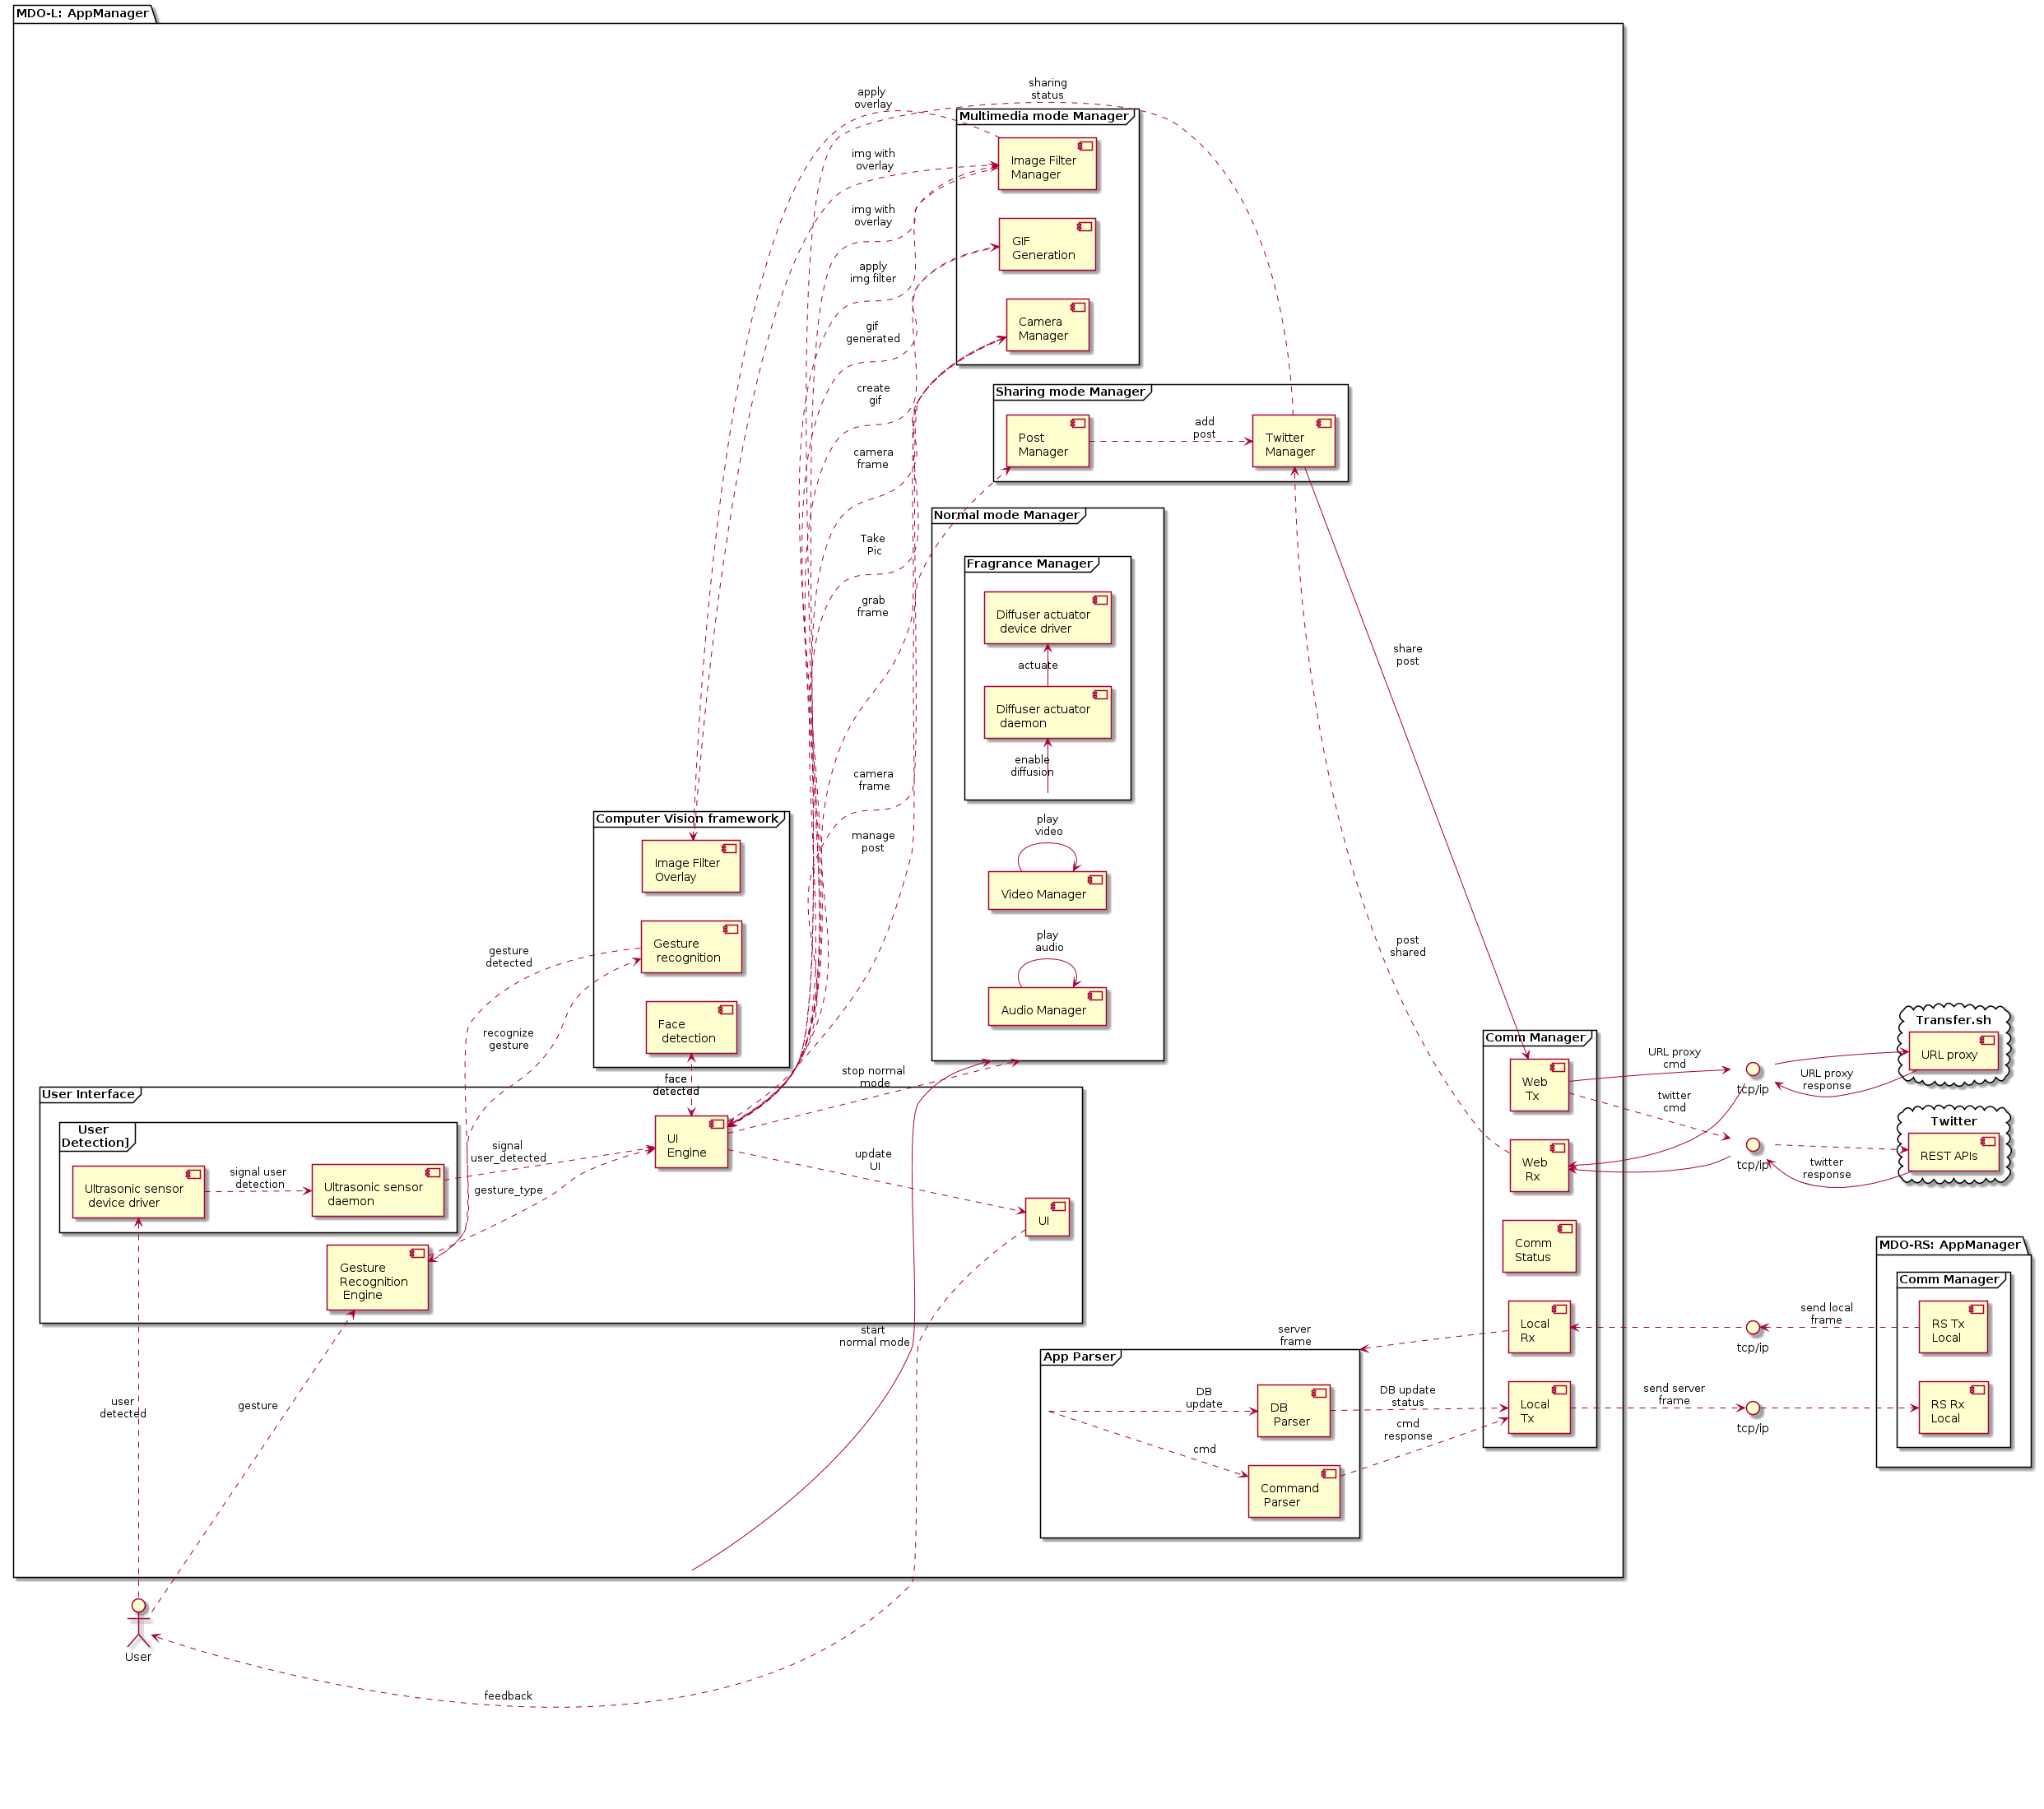
\includegraphics[width=1.03\columnwidth]{./img/component-diag-local.png}
  \caption{\gls{sw} architecture: component diagram --- \texttt{Local system}}%
\label{fig:component-diag-local}
\end{figure}

%At program
% startup --- \texttt{Idle} state --- the peripherals are initialized (interrupts, PCA, I2C, timer for tick
% generated interrupts) and the program waits for events, going into sleep
% mode.
% 
% When a key is pressed, the external interrupt \texttt{INTO} signals this
% event right away to the CPU awaking it up triggering the execution of
% \texttt{ISR\_Key\_Press}. This ISR checks which key was pressed by reading it
% from the I/O expander via I2C, pushes the associated code to
% \texttt{keycode\_fifo} --- a circular \gls{fifo} buffer --- and flags it to the CPU, enabling \texttt{keycode\_avail}.
% 
% The CPU is awaked regularly to check if any keycode is available. If it is, it
% triggers the execution of \texttt{ISR\_IR\_emit}, clearing the flag
% \texttt{keycode\_avail}, popping the keycode from \texttt{keycode\_fifo} and
% sending it via IR circuitry (\texttt{ir\_send(keycode)}).
% %
%   \vspace{-5mm}
% %  
% \begin{figure}[htb!]
% \centering
%     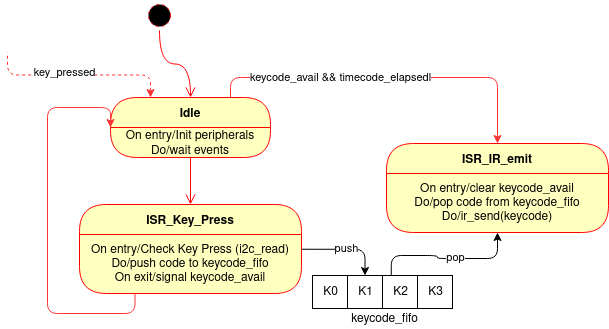
\includegraphics[width=0.7\columnwidth]{./img/state-mach.png}
%   \caption{TV remote state machine diagram}%
% \label{fig:state-mach}
% \end{figure}
% 
% Fig.~\ref{fig:i2cread-flow} presents the flowchart for reading from the I/O expander via i2c
% 
% \begin{figure}[htb!]
% \centering
%     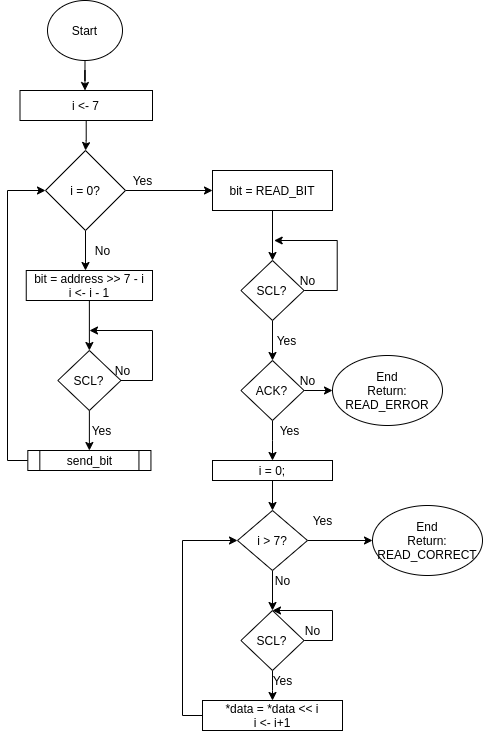
\includegraphics[width=0.7\columnwidth]{./img/i2c_read_flowchart.png}
%   \caption{I2C Read Flowchart}%
% \label{fig:i2cread-flow}
% \end{figure}
% %
%   \vspace{-5mm}
% %  
\section{Software interfaces definition}
\label{sec:sw-interf-def}
%- Define the APIs in detail:
%  - header files with:
%    - functions prototypes
%    - data structure declarations
%    - class declarations
%
% From the state machine diagram (Fig.~\ref{fig:state-mach}) the softwares modules
% and data structures can be infered. The data structure is \texttt{keycode\_fifo},
% a circular buffer to manage the keycodes produced and consumed. The modules are
% \texttt{i2c}, \texttt{ir} and \texttt{fifo} for determing the key pressed,
% transmitting the keycode and managing the \gls{fifo} buffer. Enumerations are
% added for keycodes and errors listing.
% 
% An example of the \gls{api} can be seen in Listing~\ref{lst:api}, using builtin documentation.
% %
% \lstinputlisting[language=c, firstline=1,caption={\gls{api} example with
%   builtin documentation},label=lst:api,
% style=customc]{./listing/api.h}%

\section{Start-up/shutdown process specification}
\label{sec:startup-shutdown}
%As highlighted in Fig.~\ref{fig:state-mach}, the process starts with battery
%power being supplied to the system, going into sleep mode and waiting for
%events, minimizing power consumption. However, there is still residual power
%being drawn. This could be overcome by placing a power button for the remote
%itself, but with the inconvenience of MCU reset and the initial delays
%associated. The shutdown results from batteries disconnection.\

\section{Error handling specification}
\label{sec:error-handling-specification}
%Every system is prone to glitches, bugs and errors, thus, requiring it to be
%handled. Errors should be handled gracefully by creating error handling
%routines, which try to circumvent them and provide feedback.
%
%For extreme cases, where this is not possible, the watchdog timer should be
%enabled to help the system recover from crashes. However, this is a last resort,
%as constant reboots --- sign of a bad design --- are inadmissible and will
%frustrate the user.
%
%The error handling routines can be built into the design by considering return
%codes and asserts from function calls, e.g., \texttt{int i2c\_read(char *byte)},
%where \texttt{0} signals success and otherwise an error was encountered. Thus,
%good design eases error-handling specification and should be an aspect to keep
%in mind in this phase.
%%
%  \vspace{-5mm}
%%% Local Variables:
%%% mode: latex
%%% TeX-master: "../../../dissertation"
%%% End:
